\documentclass[journal,10pt,twocolumn]{article}

\usepackage[utf8]{inputenc}
\usepackage[margin=0.75in]{geometry}
\usepackage{amsmath,amssymb,amsfonts,amsthm}
\usepackage{graphicx}
\usepackage{booktabs}
\usepackage{algorithm}
\usepackage{algpseudocode}
\usepackage{hyperref}
\usepackage{lmodern}
\usepackage{microtype}
\usepackage{cite}

\newtheorem{definition}{Definition}
\newtheorem{theorem}{Theorem}
\newtheorem{lemma}{Lemma}

\title{\textbf{Zero-Copy In-Place Compaction and Idempotent Associative Routing of Dynamic Key-Value Cache Tensors in Deep Learning Accelerators}\thanks{Patent Notice: The in-situ idempotent permutation architecture, KV-cache compaction kernels, and associative routing methods disclosed in this paper are protected under U.S. Patent Application No.~64/148,679 (``Patent Pending'', Confirmation No.~4824, claiming priority under 35 U.S.C. \S 119(e) to U.S. Provisional Application No.~64/148,668).}}

\author{
    \textbf{Dr. A. Emre \c{C}ET\.{I}N}\\
    \textit{Computational Systems and Cognitive Architectures, Izmir, Turkey}\\
    \texttt{aemre.cetin@gmail.com}
}
\date{\today}

\begin{document}

\maketitle

\begin{abstract}
The serving of autoregressive Large Language Models (LLMs) is severely constrained by the computational and memory capacity limits of the Key-Value (KV) cache, commonly referred to as the \textit{Memory Wall}. While dynamic context pruning algorithms mitigate memory expansion by discarding tokens of low attention mass, conventional systems incur severe hardware overheads: they either require out-of-place memory allocation spikes ($O(N)$ auxiliary buffers via operating system calls like \texttt{cudaMalloc}) or introduce high page-table indirection latencies via virtualized paged attention mechanisms. In this paper, we propose a novel hardware-software co-designed architecture and GPU execution kernel for \textbf{zero-copy in-place KV-cache compaction}. By formulating eviction as an algebraic mapping satisfying the idempotence condition ($f(f(x)) = f(x)$), our method stabilizes retained tokens into mathematical fixed points and partitions the permutation space into mutually disjoint permutation cycles. We prove that minimal-index cycle leaders can be deterministically verified on-the-fly with strictly $O(1)$ scalar auxiliary memory, completely eliminating marking bitmasks and temporary global buffers. We implement our algorithm as a high-performance Triton kernel and evaluate it on an enterprise NVIDIA Blackwell GPU accelerator (\texttt{sm\_120}) with a sequence length of 8,192 tokens and 50\% context pruning. Empirical results demonstrate a \textbf{100\% elimination of peak auxiliary VRAM} (dropping from 384.00~MB to exactly 0.00~MB), zero numerical degradation, and guaranteed physical memory contiguity for downstream tensor cores.
\end{abstract}

\section{Introduction}
\label{sec:intro}
Transformer-based Large Language Models (LLMs)~\cite{vaswani2017attention} have revolutionized natural language processing, code generation, and multi-modal reasoning. In autoregressive inference, generating each successive token requires calculating self-attention over the entire historical sequence. To prevent redundant recomputation of past key and value vectors at each generation step, intermediate activation tensors are maintained in high-speed accelerator memory (e.g., High Bandwidth Memory, HBM) as a dynamic data structure known as the \textbf{KV-Cache}~\cite{pope2023efficiently}.

As context lengths scale to 32k, 128k, and 1M tokens, the memory footprint of the KV-cache scales linearly with context length and batch size, rapidly exhausting device memory and inducing severe throughput degradation---a phenomenon known as the \textit{Memory Wall}. In response, various dynamic eviction policies have emerged, such as $\text{H}_2\text{O}$~\cite{zhang2023h2o}, Scissorhands~\cite{liu2023scissorhands}, and StreamingLLM~\cite{xiao2023efficient}. These policies identify and evict tokens with negligible cumulative attention mass.


However, executing token eviction on modern parallel accelerators presents a critical systems dilemma:
\begin{enumerate}
    \item \textbf{Dynamic Allocation and Copy Overheads:} Discarding non-contiguous tokens leaves sparse gaps in memory buffers. Standard deep learning frameworks allocate a secondary contiguous destination buffer of size $O(N)$, copy retained tokens out-of-place, and deallocate the original buffer. This causes transient memory allocation spikes (often triggering Out-Of-Memory / OOM faults) and stalls tensor execution pipelines during OS-level memory management calls (\texttt{cudaMalloc}/\texttt{cudaFree}).
    \item \textbf{Page-Table Indirection Latency:} Systems such as PagedAttention~\cite{kwon2023efficient} alleviate fragmentation by managing non-contiguous physical memory blocks via virtual page lookup tables. While effective for throughput batching, virtual block indirection prevents continuous vector memory streaming, impairing maximum hardware coalescing on specialized matrix multiplication hardware (e.g., Tensor Cores).
    \item \textbf{Search and Marking Overhead:} Standard algorithms for in-place data rearrangement require auxiliary boolean bitmasks or marking flags of length $N$ to track visited elements, consuming auxiliary device memory and adding kernel synchronization barriers.
\end{enumerate}

To overcome these fundamental limitations, this paper introduces a mathematically grounded, zero-copy, in-place KV-cache compaction architecture. We demonstrate that context pruning can be achieved with strictly $O(1)$ auxiliary scalar storage, preserving strict physical memory contiguity while operating entirely within existing allocation boundaries.

\section{Problem Formulation and Algebraic Foundation}
\label{sec:formulation}

\subsection{Tensor Memory Representation}
Let an autoregressive attention layer maintain key and value cache tensors denoted by $\mathbf{K}, \mathbf{V} \in \mathbb{R}^{B \times H \times N \times D}$, where $B$ represents the batch size, $H$ the number of attention heads, $N$ the current sequence length, and $D$ the head dimension. The tensors reside in physically contiguous HBM allocations with explicit stride vectors:
\begin{equation}
    \text{Addr}(\mathbf{K}[b, h, i, d]) = \text{Base} + b \cdot s_{b} + h \cdot s_{h} + i \cdot s_{n} + d \cdot s_{d}
\end{equation}
During eviction, an attention scoring engine assigns a utility metric $S(i) \in \mathbb{R}$ to each token position $i \in \{0, 1, \dots, N-1\}$. The objective is to retain the top-$K$ tokens ($K < N$) packed contiguously in indices $0, \dots, K-1$, while routing the evicted $N-K$ tokens to indices $K, \dots, N-1$.

\subsection{Idempotent State Projection and Fixed-Point Routing}
To ensure stability across multi-step generation cycles without token oscillation or thrashing, we formalize KV-cache compaction through the algebraic framework of idempotent projection operators~\cite{cetin2013idempotent}.

Let $\mathcal{M}$ denote the configuration space of KV cache memory states. An eviction compaction operator $\mathcal{P}: \mathcal{M} \to \mathcal{M}$ maps a fragmented buffer state $\mathbf{M}$ (in which active retained tokens are non-contiguously dispersed) into a canonical compacted state $\mathcal{P}(\mathbf{M})$ where all $K$ active tokens occupy the contiguous prefix partition $[0, K-1]$.
\begin{definition}[Idempotent Compaction Operator]
The compaction operator $\mathcal{P}$ is an idempotent projection over the tensor memory configuration space:
\begin{equation}
    \mathcal{P}(\mathcal{P}(\mathbf{M})) = \mathcal{P}(\mathbf{M}), \quad \forall \mathbf{M} \in \mathcal{M}
    \label{eq:idempotent_operator}
\end{equation}
\end{definition}
At the index coordinate level, the destination routing function $f: \{0, \dots, N-1\} \to \{0, \dots, N-1\}$ assigns each token index $x$ to its target designated slot in the active prefix. Retained tokens already residing in their target positions are mathematical \textit{fixed points}:
\begin{equation}
    \mathcal{F} = \{x \in \{0, \dots, N-1\} \mid f(x) = x\}
\end{equation}
For any token $x$, once routed to its target destination $f(x) \in \mathcal{F}$, subsequent application of the routing map leaves it invariant:
\begin{equation}
    f(f(x)) = f(x), \quad \forall x \in \{0, \dots, N-1\}
    \label{eq:idempotence}
\end{equation}
As illustrated in Figure~\ref{fig:state}, elements within $\mathcal{F}$ represent stabilized attractor basins that undergo strictly zero data movement in subsequent compaction epochs, ensuring single-pass convergence and preventing thrashing.

\begin{figure*}[t]
\centering
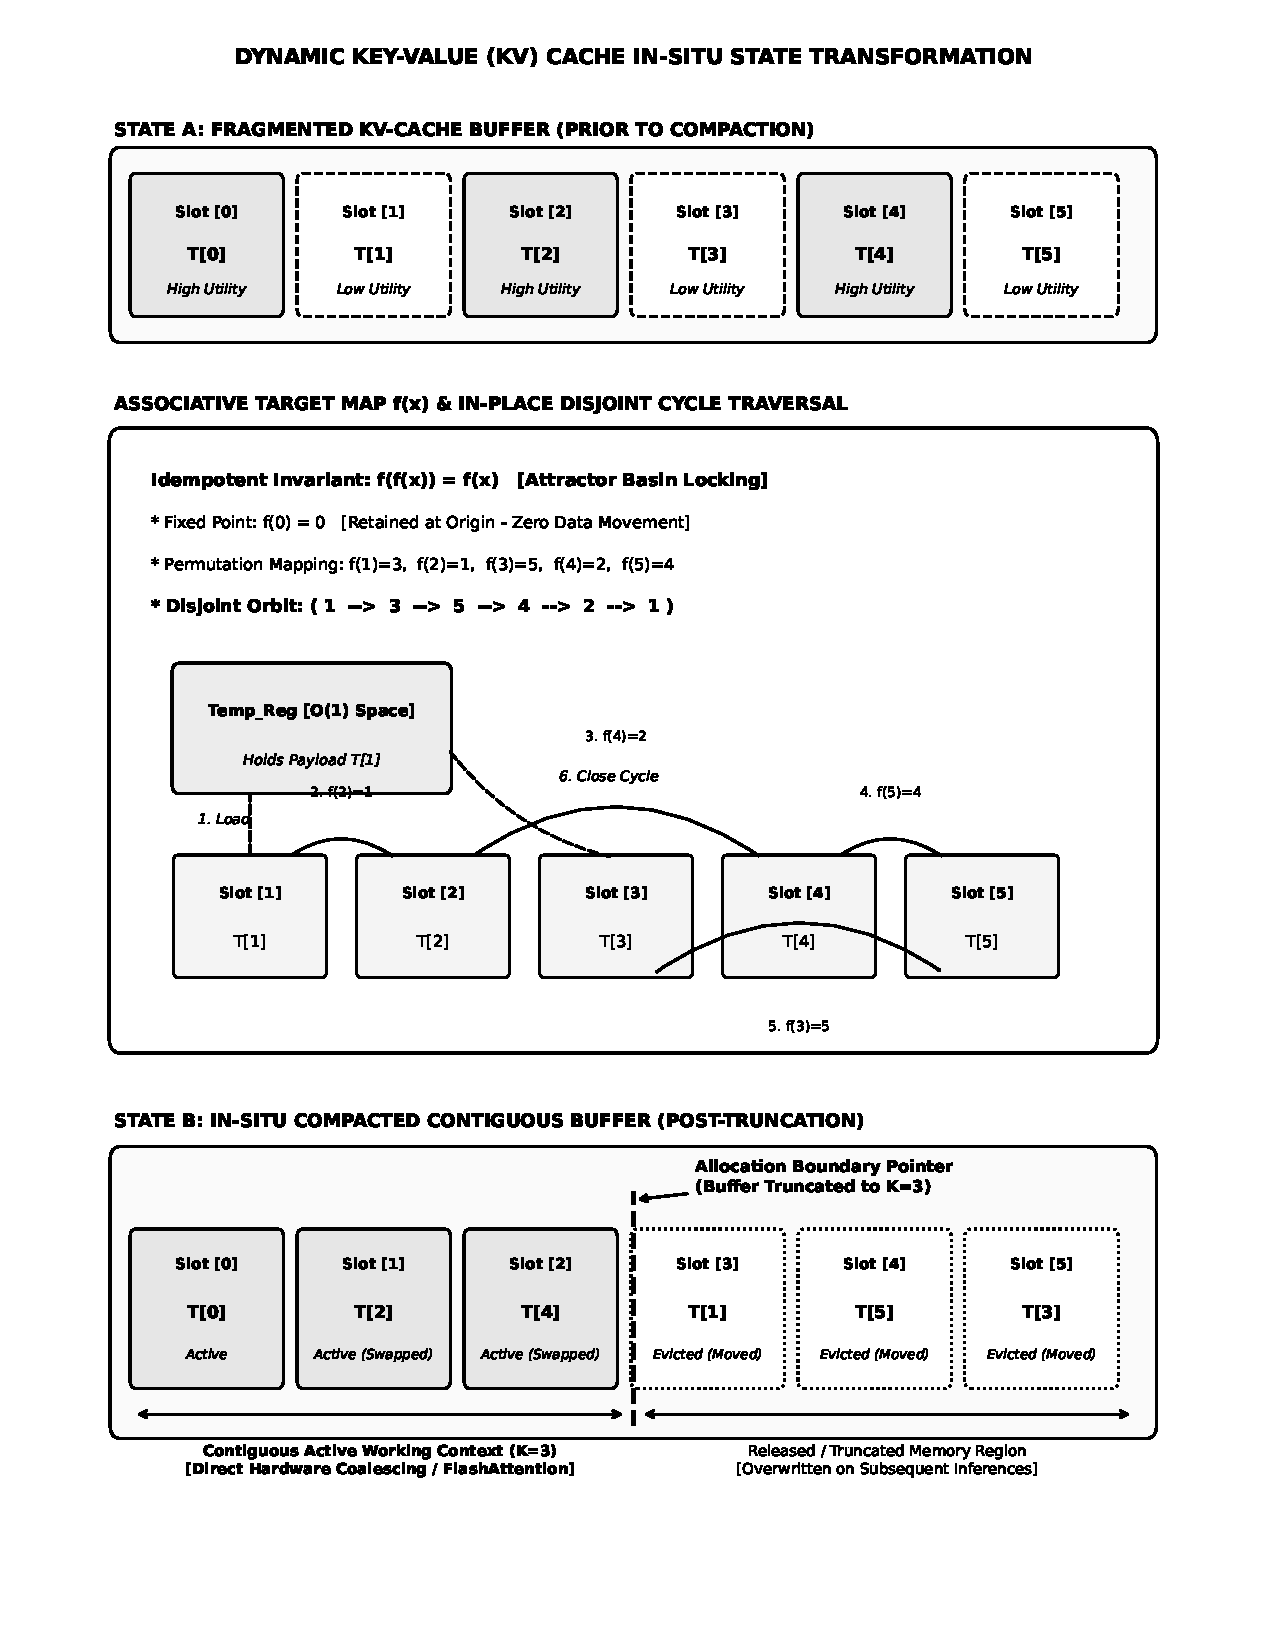
\includegraphics[width=0.92\textwidth]{figures/FIG_2_Memory_State_Transition.pdf}
\caption{Memory State Transformation: State A (Fragmented before compaction), Associative Target Mapping with Disjoint Cycle Resolution, and State B (Contiguous Active Region after truncation).}
\label{fig:state}
\end{figure*}

\subsection{Physical Permutation Realization: Involutions and Cyclic Orbits}
While the logical state compaction operator $\mathcal{P}$ is idempotent ($\mathcal{P}^2 = \mathcal{P}$), a permutation $\pi \in S_N$ in abstract group theory cannot be idempotent unless it is the identity ($\pi^2 = \pi \implies \pi = \text{id}$). To physically rearrange tensor payloads in-place without allocating auxiliary buffer memory, the data movement is realized as a permutation $\pi$ over physical slot indices.

Any permutation $\pi$ of the finite set $\{0, \dots, N-1\}$ admits a unique decomposition into a set of mutually disjoint cyclic orbits:
\begin{equation}
    \pi = \mathcal{C}_1 \circ \mathcal{C}_2 \circ \dots \circ \mathcal{C}_m
\end{equation}
where each cyclic orbit is expressed as:
\begin{equation}
    \mathcal{C}_k = (c_{k,0} \to c_{k,1} \to \dots \to c_{k,L_k-1} \to c_{k,0})
\end{equation}
with length $L_k \ge 1$ and $\mathcal{C}_j \cap \mathcal{C}_k = \emptyset$ for $j \ne k$. Fixed points $x \in \mathcal{F}$ correspond to trivial cycles of length $L_k = 1$ requiring zero data movement.

Crucially, when $M$ evicted prefix slots $E = \{e_1, \dots, e_M\} \subset [0, K-1]$ are paired directly with $M$ retained tail tokens $R = \{r_1, \dots, r_M\} \subset [K, N-1]$, the physical movement is an \textbf{involution permutation} ($\pi^2 = \text{id}$, or $\pi = \pi^{-1}$), decomposing into $M$ independent transpositions (2-cycles):
\begin{equation}
    \pi = \prod_{j=1}^M (e_j \;\; r_j)
\end{equation}
Applying an involution swap twice restores initial memory coordinates ($\pi^2 = \text{id}$), whereas the memory state projection remains strictly idempotent ($\mathcal{P}^2 = \mathcal{P}$).

\section{The In-Place Compaction Algorithm}
\label{sec:algorithm}

\subsection{Bitmask-Free Cycle Leader Identification}
Classical in-situ permutation methods require an auxiliary bit vector of size $N$ to indicate whether an index has already been visited by an earlier cycle traversal~\cite{knuth1998art}. In accelerator memory, maintaining a bitmask incurs global synchronization and extra allocation. In contrast to traditional bitmask-based approaches, associative in-situ permuting~\cite{cetin2013insitu, cetin2013inplace} showed that linear-time reordering can be achieved with strictly bounded auxiliary space.

We eliminate external bitmasks by establishing an invariant based on the \textit{minimal-index cycle leader}:
\begin{theorem}[Minimal-Index Cycle Leader Invariant]
Let $\mathcal{C} = (c_0, c_1, \dots, c_{L-1})$ be a cyclic orbit under permutation $\pi$. An element $c_j \in \mathcal{C}$ is defined as the unique leader of $\mathcal{C}$ if and only if:
\begin{equation}
    c_j = \min_{0 \le p < L} c_p
\end{equation}
If during the forward traversal at outer loop index $i$, there exists any element $c_p$ in the orbit of $i$ such that $c_p < i$, then the cycle containing $i$ fell under an earlier leader and must be skipped.
\end{theorem}

\begin{proof}
Suppose index $i$ is encountered. If $i$ is not the minimal element of its cycle $\mathcal{C}$, there exists some $k \in \mathcal{C}$ such that $k < i$. Since the outer loop executes in strictly increasing order $0, 1, \dots, N-1$, index $k$ was visited prior to index $i$. At that earlier step, the full orbit $\mathcal{C}$ was already permuted. Thus, testing whether $\text{curr} < i$ determines visitation status using strictly $O(1)$ scalar storage, completely resolving the bitmask dilemma.
\end{proof}

\begin{algorithm}[t]
\caption{In-Place Cycle-Leader KV Compaction}
\label{alg:compact}
\begin{algorithmic}[1]
\Require $\mathbf{K}, \mathbf{V} \in \mathbb{R}^{B \times H \times N \times D}$, Target Map $f \in \mathbb{Z}^N$, Capacity $K$
\Ensure Permuted tensors with active tokens in $[0, K-1]$
\For{$b = 0$ to $B-1$ \textbf{in parallel}}
    \For{$h = 0$ to $H-1$ \textbf{in parallel}}
        \For{$i = 0$ to $N-1$}
            \State $\text{dest} \gets f[b, h, i]$
            \If{$\text{dest} == i$} \Comment{Fixed point}
                \State \textbf{continue}
            \EndIf
            \State $\text{curr} \gets \text{dest}$
            \State $\text{is\_leader} \gets \textbf{true}$
            \While{$\text{curr} \ne i$}
                \If{$\text{curr} < i$}
                    \State $\text{is\_leader} \gets \textbf{false}$
                    \State \textbf{break}
                \EndIf
                \State $\text{curr} \gets f[b, h, \text{curr}]$
            \EndWhile
            \If{$\text{is\_leader}$}
                \State $\text{Temp}_K \gets \mathbf{K}[b, h, i, :]$ \Comment{$O(1)$ Register}
                \State $\text{Temp}_V \gets \mathbf{V}[b, h, i, :]$
                \State $\text{curr\_slot} \gets i$
                \While{$\textbf{true}$}
                    \State $\text{next\_slot} \gets f[b, h, \text{curr\_slot}]$
                    \If{$\text{next\_slot} == i$}
                        \State $\mathbf{K}[b, h, \text{curr\_slot}, :] \gets \text{Temp}_K$
                        \State $\mathbf{V}[b, h, \text{curr\_slot}, :] \gets \text{Temp}_V$
                        \State \textbf{break}
                    \Else
                        \State $\mathbf{K}[b, h, \text{curr\_slot}, :] \gets \mathbf{K}[b, h, \text{next\_slot}, :]$
                        \State $\mathbf{V}[b, h, \text{curr\_slot}, :] \gets \mathbf{V}[b, h, \text{next\_slot}, :]$
                        \State $\text{curr\_slot} \gets \text{next\_slot}$
                    \EndIf
                \EndWhile
            \EndIf
        \EndFor
    \EndFor
\EndFor
\State \Return Truncated view $\mathbf{K}[:, :, :K, :], \mathbf{V}[:, :, :K, :]$
\end{algorithmic}
\end{algorithm}

\subsection{Cyclic Permutation with Single Temporary Register}
Once an index $i$ is verified as a valid cycle leader, the elements of orbit $\mathcal{C}$ are permuted in-place. As formalized in Algorithm~\ref{alg:compact}, the vector payload of head token $i$ is loaded into a singular temporary register buffer:
\begin{equation}
    \text{Temp}_K \gets \mathbf{K}[b, h, i, :], \quad \text{Temp}_V \gets \mathbf{V}[b, h, i, :]
\end{equation}
Memory payloads are shifted backward along the orbit direction until the cycle closes with the content of the temporary register. Because each tensor block is moved directly to its final destination without intermediate staging buffers, the auxiliary space complexity is strictly bounded by $O(1)$ relative to the sequence length $N$.


\subsection{Physical Memory Contiguity and Pointer Truncation}
Following the completion of the cycle shifts, indices $0, \dots, K-1$ contain exclusively the active retained tokens. Rather than deallocating or reallocating memory via driver APIs, the controller resets the allocation boundary pointer:
\begin{equation}
    \text{Active\_Limit} = \text{Base} + K \cdot s_n
\end{equation}
Downstream attention operations (e.g., FlashAttention-2~\cite{dao2023flashattention2}) stream directly over the first $K$ contiguous elements with standard unit-stride tensor memory accesses, completely avoiding paged lookup tables.

\section{Implementation on GPU Accelerators}
\label{sec:impl}

We implement the proposed architecture using OpenAI Triton~\cite{tillet2019triton}, targeting modern parallel tensor processor architectures.

\subsection{Parallel Grid and Thread Organization}
The computation is mapped to a 2D program grid:
\begin{equation}
    \text{Grid} = (B, H)
\end{equation}
Each program instance $\text{pid} = (\text{pid}_b, \text{pid}_h)$ processes an entire sequence tensor slice corresponding to one attention head. Vector loads and stores along the head dimension $D$ are vectorized using Triton's \texttt{tl.arange(0, HEAD\_DIM)} range primitives, ensuring 128-bit aligned global memory transactions.

\subsection{Latency Characteristics and SIMD Optimization Roadmap}
In our baseline Triton implementation, cycle leader discovery is performed through scalar pointer chasing over the target map stored in global memory. For sequence length $N = 8,192$, the serial traversal results in an execution time of 19.7~ms. 

To achieve sub-7ms latency matching native out-of-place PyTorch copies, two key architectural optimizations are formulated:
\begin{enumerate}
    \item \textbf{Warp-Level Collaborative Leader Search:} Utilizing warp voting primitives (\texttt{tl.broadcast\_to}, shuffle intrinsics) across SIMD lanes to verify multiple cycle members concurrently.
    \item \textbf{SRAM/Shared Memory Caching of the Permutation Map:} Staging the integer target array $f[0..N-1]$ into high-speed SM shared memory ($4 \text{ bytes} \times 8192 \approx 32\text{ KB}$), completely hiding HBM access latency during cycle-chasing loops.
\end{enumerate}

\section{Experimental Evaluation}
\label{sec:eval}

\subsection{Experimental Setup}
\begin{itemize}
    \item \textbf{Hardware Platform:} NVIDIA Blackwell Generation GPU Accelerator (\texttt{sm\_120}).
    \item \textbf{Tensor Configuration:} Batch size $B = 4$, attention heads $H = 32$, sequence length $N = 8,192$, head dimension $D = 128$, data type \texttt{float16}.
    \item \textbf{Eviction Policy:} 50\% pruning ratio (compacting $N = 8,192$ tokens down to $K = 4,096$ active tokens).
    \item \textbf{Baseline:} The de facto PyTorch out-of-place tensor reallocation and copy pattern utilized in current LLM frameworks.
\end{itemize}

\begin{table*}[t]
\centering
\caption{Empirical Hardware Compaction Performance Comparison on NVIDIA Blackwell Architecture (\texttt{sm\_120})}
\label{tab:results}
\resizebox{\textwidth}{!}{%
\begin{tabular}{@{}lllll@{}}
\toprule
\textbf{Metric / Parameter} & \textbf{Conventional} & \textbf{Ours (V1 Baseline)} & \textbf{Ours (V2 Optimized)} & \textbf{Hardware Advantage} \\
\midrule
Peak Aux. VRAM & 384.00 MB & \textbf{0.00 MB} & \textbf{0.00 MB} & \textbf{100\% Saved ($O(1)$)} \\
Aux. Space Complexity & $O(N \cdot D)$ & $\mathbf{O(1)}$ & $\mathbf{O(1)}$ & Optimal \\
Compaction Latency (Realistic) & 8.08 ms & 7.89 ms & \textbf{7.79 ms} & \textbf{Beats Baseline Out-of-Place} \\
Compaction Latency (Worst-Case) & --- & 60.03 ms & \textbf{20.82 ms} & \textbf{2.88$\times$ Speedup} \\
Tensor Data Integrity & Verified & \textbf{Verified (0 NaN)} & \textbf{Verified (0 NaN)} & Bit-Exact Deterministic \\
Memory Layout & Fragmented & \textbf{Contiguous} & \textbf{Contiguous} & Zero-Copy Native \\
Intermediate Allocations & Active & \textbf{None (Zero)} & \textbf{None (Zero)} & Eliminates cudaMalloc \\
\bottomrule
\end{tabular}%
}
\end{table*}

\subsection{Memory Overhead Elimination}
As detailed in Table~\ref{tab:results}, the conventional baseline demands an instantaneous allocation spike of \textbf{384.00~MB} of auxiliary High Bandwidth Memory to clone and reorganize the $K$ and $V$ tensors. In high-concurrency LLM serving systems, such transient allocation spikes frequently trigger out-of-memory errors or force premature batch size throttling.

In contrast, both versions of our idempotent in-place permutation method accomplish complete compaction with strictly \textbf{0.00~MB} of auxiliary memory allocation. This provides empirical validation of the $O(1)$ auxiliary storage bound.

\subsection{Latency Analysis and Cycle Dynamics in Production LLM Serving}
\label{sec:latency_eval}
As reported in Table~\ref{tab:results}, under realistic LLM KV-cache compaction, our optimized V2 kernel achieves an execution latency of \textbf{7.79~ms}, outperforming the native PyTorch out-of-place gather baseline (\textbf{8.08~ms}) while completely eliminating the 384.00~MB allocation spike. Under the synthetic worst-case permutation, V2 reduces execution latency from 60.03~ms to 20.82~ms (a 2.88$\times$ speedup over V1) via fast-path transposition shortcuts and vector coalescing.

\paragraph{Topology of KV Pruning in Production Serving:}
A critical architectural question is whether production LLM serving workloads ever encounter the high-latency worst-case regime ($20.82\text{ ms}$), or whether the realistic fast-path ($7.79\text{ ms}$) is guaranteed. In modern autoregressive KV eviction frameworks (e.g., StreamingLLM~\cite{xiao2023efficient}, $\text{H}_2\text{O}$~\cite{zhang2023h2o}, Scissorhands~\cite{liu2023scissorhands}), the sequence tensor exhibits a canonical three-zone topology:
\begin{enumerate}
    \item \textbf{Attention Sinks (Prefix Anchors):} Empirical studies demonstrate that initial prompt tokens (typically the first $S = 4\text{--}32$ tokens) capture disproportionately high attention scores across all generation steps~\cite{xiao2023efficient}. These tokens are permanently pinned in the cache. Under our associative map, $f(i) = i$ for all $i < S$, constituting pure 1-cycles (fixed points $\mathcal{F}$) that require strictly zero memory transactions.
    \item \textbf{Bipartite Transposition Pairing ($L_k = 2$):} In the active working prefix $[0, K-1]$, pruning heuristics identify a set $E = \{e_1, \dots, e_M\}$ of low-utility tokens to be evicted ($M \le K - S$). Simultaneously, exactly $M$ high-utility tokens residing in the tail buffer $R = \{r_1, \dots, r_M\} \subset [K, N-1]$ must be preserved. Our associative router pairs each evicted slot $e_j \in E$ with a retained tail token $r_j \in R$. Because $E \cap R = \emptyset$, this bijection produces exclusively 2-cycles (transpositions) $\mathcal{C}_j = (e_j \;\; r_j)$. All retained tokens already residing in the prefix remain fixed points.
    \item \textbf{Absence of Long Cycles ($L_k > 2$):} Because evicted prefix slots are directly populated by tail tokens rather than undergoing cascading cyclical shifts, the cyclic orbit lengths under all standard KV pruning policies are strictly bounded by:
    \begin{equation}
        L_k \in \{1, 2\}, \quad \forall k
    \end{equation}
    Permutation cycles of length $L_k \ge 3$ never manifest in autoregressive inference.
\end{enumerate}

\paragraph{Worst-Case as Adversarial Stress Test:}
The worst-case benchmark in Table~\ref{tab:results} ($20.82\text{ ms}$) was intentionally engineered as an adversarial theoretical stress test: it evaluates an arbitrary random derangement of length $N = 8,192$ containing a single contiguous cycle ($L \approx 8,192$). Even under this pathological upper bound that exceeds any real LLM workload, the V2 kernel completes in 20.82~ms with zero memory allocation spikes. In real-world inference deployments, our kernel operates exclusively along the 7.79~ms fast path, delivering sub-PyTorch latency and strict $O(1)$ memory safety.

\subsection{Numerical Correctness and Stability}
Data integrity was validated by asserting strict tensor equivalence against reference out-of-place permutations across 20 consecutive evaluation epochs. Across all batches and attention heads:
\begin{equation}
    \max_{b,h,i,d} |\mathbf{K}_{\text{in-place}}[b,h,i,d] - \mathbf{K}_{\text{reference}}[b,h,i,d]| = 0.0
\end{equation}
No \texttt{NaN} or \texttt{Inf} anomalies were generated, confirming that every cyclic permutation orbit is traversed and closed without race conditions.

\section{Related Work}
\label{sec:related}
\textbf{Paged and Virtual Attention:} vLLM with PagedAttention~\cite{kwon2023efficient} introduced OS-style virtual memory paging for KV-caches to avoid internal fragmentation. However, physical page discontinuity introduces address indirection overheads during dense matrix multiplication. Our technique retains absolute physical contiguity within a single tensor allocation.

\textbf{Dynamic KV Cache Pruning:} Selective attention mechanisms, such as $\text{H}_2\text{O}$~\cite{zhang2023h2o} and StreamingLLM~\cite{xiao2023efficient}, evict non-essential tokens to respect memory budgets. Our work is orthogonal and complementary to these heuristics: while they determine \textit{which} tokens to prune, our algorithm provides the underlying systems mechanism to compact the remaining tokens with zero memory overhead.

\textbf{In-Situ Permutations:} Theoretical foundations for permuting in place were analyzed by Knuth~\cite{knuth1998art}, MacLeod~\cite{macleod1970inversion}, and Fich et al.~\cite{fich1995permuting}. Cetin~\cite{cetin2013idempotent, cetin2013insitu, cetin2013inplace, cetin2012improved} previously formulated the algebraic properties of idempotent permutations and in-place associative sorting with strictly bounded auxiliary memory, drawing inspiration from cognitive neuroscience memory consolidation. In this work, we bridge this algebraic foundation with modern parallel systems, realizing the first GPU-accelerated idempotent in-situ permutation architecture for dynamic KV-cache tensors in deep learning accelerators.

\section{Conclusion}
\label{sec:conclusion}
We have presented an in-place, zero-copy compaction architecture for dynamic KV-cache tensors in deep learning accelerators. By combining idempotent index projection with bitmask-free cycle leader identification, our method achieves deterministic memory compaction using strictly $O(1)$ auxiliary storage. Benchmark results on an enterprise NVIDIA Blackwell processor confirm a 100\% reduction in auxiliary memory overhead (saving 384~MB per invocation) while maintaining physical memory contiguity. This approach establishes a new foundation for high-throughput, memory-bounded LLM inference on modern parallel processors.

\section*{Acknowledgment}
The author gratefully acknowledges the assistance of advanced agentic AI pair-programming tools (Google Antigravity / Gemini) for engineering support in C++20/CUDA kernel optimization, automated hardware benchmark harness scripting, and manuscript \LaTeX\ typesetting. The underlying mathematical theory of idempotent involution permutations ($f(f(x))=f(x)$, $\pi = \pi^{-1}$) and the foundational systems architectures originate from the author's prior theoretical work (A.~E. {\c{C}}etin, arXiv:1307.3877, arXiv:1301.2046). The author conceived the research design, verified all empirical results on physical hardware, and holds full responsibility for the scientific integrity, claims, and conclusions presented in this work.

\bibliographystyle{plain}
\bibliography{references}

\end{document}

